%===============================================================================
% LaTeX sjabloon voor de bachelorproef toegepaste informatica aan HOGENT
% Meer info op https://github.com/HoGentTIN/latex-hogent-report
%===============================================================================

\documentclass[dutch,dit,thesis]{hogentreport}

% TODO:
% - If necessary, replace the option `dit`' with your own department!
%   Valid entries are dbo, dbt, dgz, dit, dlo, dog, dsa, soa
% - If you write your thesis in English (remark: only possible after getting
%   explicit approval!), remove the option "dutch," or replace with "english".

\usepackage{lipsum} % For blind text, can be removed after adding actual content

%% Pictures to include in the text can be put in the graphics/ folder
\graphicspath{{../graphics/}}

%% For source code highlighting, requires pygments to be installed
%% Compile with the -shell-escape flag!
%% \usepackage[chapter]{minted}
%% If you compile with the make_thesis.{bat,sh} script, use the following
%% import instead:
\usepackage[chapter,outputdir=../output]{minted}
\usemintedstyle{solarized-light}

%% Formatting for minted environments.
\setminted{%
    autogobble,
    frame=lines,
    breaklines,
    linenos,
    tabsize=4
}

%% Ensure the list of listings is in the table of contents
\renewcommand\listoflistingscaption{%
    \IfLanguageName{dutch}{Lijst van codefragmenten}{List of listings}
}
\renewcommand\listingscaption{%
    \IfLanguageName{dutch}{Codefragment}{Listing}
}
\renewcommand*\listoflistings{%
    \cleardoublepage\phantomsection\addcontentsline{toc}{chapter}{\listoflistingscaption}%
    \listof{listing}{\listoflistingscaption}%
}

% Other packages not already included can be imported here

%%---------- Document metadata -------------------------------------------------
% TODO: Replace this with your own information
\author{Wout De Temmerman}
\supervisor{Martijn Saelens}
\cosupervisor{Andy Van Maele}
\title{IPv6-verbindingen: Automatisering van tunnelconfiguratie met Ansible}
\academicyear{\advance\year by -1 \the\year--\advance\year by 1 \the\year}
\examperiod{1}
\degreesought{\IfLanguageName{dutch}{Professionele bachelor in de toegepaste informatica}{Bachelor of applied computer science}}
\partialthesis{false} %% To display 'in partial fulfilment'
%\institution{Internshipcompany BVBA.}

%% Add global exceptions to the hyphenation here
\hyphenation{back-slash}

%% The bibliography (style and settings are  found in hogentthesis.cls)
\addbibresource{bachproef.bib}            %% Bibliography file
\addbibresource{../voorstel/voorstel.bib} %% Bibliography research proposal
\defbibheading{bibempty}{}

%% Prevent empty pages for right-handed chapter starts in twoside mode
\renewcommand{\cleardoublepage}{\clearpage}

\renewcommand{\arraystretch}{1.2}

%% Content starts here.
\begin{document}

%---------- Front matter -------------------------------------------------------

\frontmatter

\hypersetup{pageanchor=false} %% Disable page numbering references
%% Render a Dutch outer title page if the main language is English
\IfLanguageName{english}{%
    %% If necessary, information can be changed here
    \degreesought{Professionele Bachelor toegepaste informatica}%
    \begin{otherlanguage}{dutch}%
       \maketitle%
    \end{otherlanguage}%
}{}

%% Generates title page content
\maketitle
\hypersetup{pageanchor=true}

%%=============================================================================
%% Voorwoord
%%=============================================================================

\chapter*{\IfLanguageName{dutch}{Woord vooraf}{Preface}}%
\label{ch:voorwoord}

%% TODO:
%% Het voorwoord is het enige deel van de bachelorproef waar je vanuit je
%% eigen standpunt (``ik-vorm'') mag schrijven. Je kan hier bv. motiveren
%% waarom jij het onderwerp wil bespreken.
%% Vergeet ook niet te bedanken wie je geholpen/gesteund/... heeft

Al van jongs af aan ben ik gefascineerd door de werking van netwerken en de essentiële rol die ze spelen in onze digitale wereld.  
Tijdens mijn opleiding Toegepaste Informatica aan HOGENT werd mijn interesse hierin verder aangewakkerd.  
Een uitspraak van mijn lector Netwerken is me daarbij altijd bijgebleven:  

\begin{quote}
    ``Het is niet logisch dat onze school IPv6, een technologie die al geruime tijd bestaat, bespreekt in de netwerklessen, maar er zelf nog geen gebruik van maakt.''
\end{quote}

Dit onderzoek is daarom opgesteld om deze situatie op een eenvoudige manier te omzeilen en een duidelijk onderscheid te maken tussen de verschillende tunneltechnieken die hiermee gepaard gaan.\\

Bij deze wil ik graag enkele personen bedanken die een essentiële rol hebben gespeeld bij deze bachelorproef.  
Allereerst wil ik mijn co-promotor en lector, Andy Van Maele, bedanken voor zijn begeleiding, advies en waardevolle feedback gedurende dit project.  
Daarnaast ben ik mijn promotor, \textbf{\#TODO\#}, dankbaar voor zijn interesse en bereidheid om op het laatste moment nog de rol van promotor op zich te nemen.
Ook wil ik lector Bert Van Vreckem bedanken voor zijn hulp bij de opzet van de virtuele machines die nodig waren voor de proof of concept.
Tot slot wil ik ook mijn bachelorproefcoördinator, Lena De Mol, bedanken voor haar ondersteuning en hulp bij het bewaken van het verloop van de proef.  


%%=============================================================================
%% Samenvatting
%%=============================================================================

% TODO: De "abstract" of samenvatting is een kernachtige (~ 1 blz. voor een
% thesis) synthese van het document.
%
% Een goede abstract biedt een kernachtig antwoord op volgende vragen:
%
% 1. Waarover gaat de bachelorproef?
% 2. Waarom heb je er over geschreven?
% 3. Hoe heb je het onderzoek uitgevoerd?
% 4. Wat waren de resultaten? Wat blijkt uit je onderzoek?
% 5. Wat betekenen je resultaten? Wat is de relevantie voor het werkveld?
%
% Daarom bestaat een abstract uit volgende componenten:
%
% - inleiding + kaderen thema
% - probleemstelling
% - (centrale) onderzoeksvraag
% - onderzoeksdoelstelling
% - methodologie
% - resultaten (beperk tot de belangrijkste, relevant voor de onderzoeksvraag)
% - conclusies, aanbevelingen, beperkingen
%
% LET OP! Een samenvatting is GEEN voorwoord!

%%---------- Nederlandse samenvatting -----------------------------------------
%
% TODO: Als je je bachelorproef in het Engels schrijft, moet je eerst een
% Nederlandse samenvatting invoegen. Haal daarvoor onderstaande code uit
% commentaar.
% Wie zijn bachelorproef in het Nederlands schrijft, kan dit negeren, de inhoud
% wordt niet in het document ingevoegd.

\IfLanguageName{english}{%
\selectlanguage{dutch}
\chapter*{Samenvatting}
\selectlanguage{english}
}{}

%%---------- Samenvatting -----------------------------------------------------
% De samenvatting in de hoofdtaal van het document

\chapter*{\IfLanguageName{dutch}{Samenvatting}{Abstract}}

% SmartEye beheert meer dan 700 netwerklocaties, waaronder particuliere kotuitbaters, studentenvoorzieningen zoals Upkot en Xior, en onderwijsinstellingen zoals HOGENT en Artevelde. 
% De diversiteit aan infrastructuur maakt het uitrollen van netwerkupgrades uitdagend, vooral omdat elk type netwerkapparatuur een verschillende configuratie vereist. 
% Met de geplande overgang naar IPv6 staat SmartEye voor de taak om hun netwerken toekomstbestendig te maken met een geautomatiseerde oplossing. 
% Hiervoor willen ze gebruik maken van Ansible Playbooks, maar er is nog onvoldoende duidelijkheid over wat er nodig is om een goed werkend playbook op te stellen dat aan al hun eisen voldoet. 
% Dit onderzoek richt zich op het scheppen van duidelijkheid over de noodzakelijke componenten bij het opstellen van een Ansible Playbook voor de ondersteuning van IPv6 in verschillende netwerkinfrastructuren. 
% De focus ligt op het in kaart brengen van vereisten en best practices, het identificeren van mogelijke knelpunten en het onderzoeken van netwerkapparaten die extra aandacht nodig hebben voor compatibiliteit, 
% met specifieke aandacht voor de configuratie van MikroTik-toestellen, aangezien deze de backbone van het netwerk vormen.
% \\

% Onderzoek werd gedaan met een combinatie van literatuurstudie en experimentele implementatie binnen het netwerk van SmartEye toegepast. 
% Dit omvatte een analyse van de MikroTik documentatie, het opzetten van een testomgeving, het ontwikkelen en testen van Ansible Playbooks en een evaluatie van de prestaties en betrouwbaarheid van de playbooks in een realistische netwerkomgeving. 
% Uit de resultaten blijkt dat een dual-stack implementatie de beste optie is om met IPv6 te starten, aangezien dit de downtime het laagst houdt. 
% Indien SmartEye dan achteraf wilt overschakelen naar een puur IPv6 netwerk kan dit ook gedaan worden zonder opmerkelijke downtime te creëren.
% \\

% De resultaten tonen aan dat automatisering met Ansible Playbooks een effectieve manier is om de overstap naar IPv6 te ondersteunen, mits er rekening wordt gehouden met compatibiliteitsproblemen en hardwarebeperkingen. 
% Verder onderzoek kan zich richten op bredere compatibiliteitskwesties met andere netwerkfabrikanten en de integratie van beveiligingsmaatregelen binnen de IPv6-configuratie.


TODO

%---------- Inhoud, lijst figuren, ... -----------------------------------------

\tableofcontents

% In a list of figures, the complete caption will be included. To prevent this,
% ALWAYS add a short description in the caption!
%
%  \caption[short description]{elaborate description}
%
% If you do, only the short description will be used in the list of figures

\listoffigures

% If you included tables and/or source code listings, uncomment the appropriate
% lines.
% \listoftables

% \listoflistings

% Als je een lijst van afkortingen of termen wil toevoegen, dan hoort die
% hier thuis. Gebruik bijvoorbeeld de ``glossaries'' package.
% https://www.overleaf.com/learn/latex/Glossaries

%---------- Kern ---------------------------------------------------------------

\mainmatter{}

% De eerste hoofdstukken van een bachelorproef zijn meestal een inleiding op
% het onderwerp, literatuurstudie en verantwoording methodologie.
% Aarzel niet om een meer beschrijvende titel aan deze hoofdstukken te geven of
% om bijvoorbeeld de inleiding en/of stand van zaken over meerdere hoofdstukken
% te verspreiden!

%%=============================================================================
%% Inleiding
%%=============================================================================

\chapter{\IfLanguageName{dutch}{Inleiding}{Introduction}}%
\label{ch:inleiding}

\section{\IfLanguageName{dutch}{Probleemstelling}{Problem Statement}}%
\label{sec:probleemstelling}

Door de implementatie van IPv6 kan een netwerk snel futureproof worden gemaakt. 
Het is een relatief nieuwe technologie die het probleem van de gelimiteerde 32-bit adressen in IPv4 oplost door gebruik te maken van 128-bit adressen. 
Hoewel IPv6 al sinds 1998 bestaat, blijft de toepassing ervan beperkt. Dit blijkt duidelijk uit de IPv6 Support Rate-grafiek op de website van \textcite{EuropeanCommission}, 
waaruit blijkt dat in België begin 2024 59\% van de eindgebruikers toegang heeft tot IPv6, terwijl slechts 29\% van de services compatibel zijn met de technologie.
\\

Deze cijfers tonen aan dat de adoptie van IPv6 groeit aan constante snelheid, maar dat er nog steeds een duidelijke kloof bestaat tussen netwerktoegang en implementatie. 
Aangezien bedrijven en organisaties steeds vaker overschakelen op IPv6, wordt het voor toekomstige IT-professionals essentieel om hier grondige kennis over te verwerven. 
Daarom is het belangrijk dat de opleiding IPv6 een plaats geeft binnen het curriculum, zodat studenten goed voorbereid zijn op de netwerkinfrastructuur van de toekomst.
\\

Het netwerklabo op campus Schoonmeersen van HOGENT wordt frequent gebruikt voor demonstraties en proefopstellingen in de lessen Netwerken 1 tot 4. 
Echter, het labo mist een essentieel component: een IPv6-verbinding. 
Een mogelijke oplossing is het gebruik van een node op de servers van IDLab aan de UGent. 
Via deze node kan een tunnel worden opgezet, waardoor het netwerkverkeer via het UGent-netwerk – dat wél IPv6 ondersteunt – kan worden gerouteerd.
\\

Deze opstelling kan al worden gerealiseerd met een bestaand script, geschreven door dhr. Van Maele. 
Dit script legt een verbinding tussen een virtuele machine en de node in IDLab, waarbij de node fungeert als OpenVPN-server en de virtuele machine als OpenVPN-client. 
Daarnaast wordt er een Layer 2-tunnel opgezet tussen deze twee punten, waarop de OpenVPN-verbinding steunt.
Het probleem hierbij is echter dat het opzetten van deze configuratie veel tijd en moeite vergt van de lectoren, 
of zelfs niet praktisch uitvoerbaar is vanwege het gebrek aan gebruiksvriendelijkheid van het script.

\section{\IfLanguageName{dutch}{Onderzoeksvraag}{Research question}}%
\label{sec:onderzoeksvraag}

De vraag waarover dit onderzoek een oplossing probeert te vinden gaat als volgt:
Kan de opzet van een IPv6 connectie aan de hand van een tunnel geautomatiseerd worden met Ansible?

Om deze verder onder te verdelen zal er vooral onderzoek worden gedaan naar volgende vragen:
\begin{itemize}
    \item Waar liggen de essentiële verschillen tussen Layer 2 en OpenVPN tunnels?
    \item Is er een vershil op vlak van performantie?
    \item Is het mogelijk om een connectie tussen 2 netwerken op te zetten met enkel een Layer 2 tunnel?
    \item Kan het bestaande script in een Ansible Playbook worden verwerkt?
    \item Wat zijn de resultaten na het testen in effectieve omgeving?
\end{itemize}

\section{\IfLanguageName{dutch}{Onderzoeksdoelstelling}{Research objective}}%
\label{sec:onderzoeksdoelstelling}

Dit onderzoek richt zich op het in kaart brengen van de verschillen tussen deze tunnelingmethodes en het testen van mogelijke alternatieve methoden. 
Uiteindelijk wordt de meest efficiënte en correcte implementatie verwerkt in een Ansible Playbook, dat automatisch de connectie tussen beide toestellen opzet.
Deze oplossing kan dan worden toegepast bij toekomstige labo’s in het netwerklabo, zodat snel en eenvoudig een functionerende IPv6-verbinding kan worden opgezet. 
Hierdoor kunnen studenten niet alleen de theorie over IPv6 bestuderen, maar deze ook daadwerkelijk testen in een realistische omgeving.

\section{\IfLanguageName{dutch}{Opzet van deze bachelorproef}{Structure of this bachelor thesis}}%
\label{sec:opzet-bachelorproef}

% Het is gebruikelijk aan het einde van de inleiding een overzicht te
% geven van de opbouw van de rest van de tekst. Deze sectie bevat al een aanzet
% die je kan aanvullen/aanpassen in functie van je eigen tekst.

De rest van deze bachelorproef is als volgt opgebouwd:

In Hoofdstuk~\ref{ch:stand-van-zaken} wordt een overzicht gegeven van de stand van zaken binnen het onderzoeksdomein, op basis van een literatuurstudie.

In Hoofdstuk~\ref{ch:methodologie} wordt de methodologie toegelicht en worden de gebruikte onderzoekstechnieken besproken om een antwoord te kunnen formuleren op de onderzoeksvragen.

% TODO: Vul hier aan voor je eigen hoofstukken, één of twee zinnen per hoofdstuk

In Hoofdstuk~\ref{ch:conclusie}, tenslotte, wordt de conclusie gegeven en een antwoord geformuleerd op de onderzoeksvragen. Daarbij wordt ook een aanzet gegeven voor toekomstig onderzoek binnen dit domein.
\chapter{\IfLanguageName{dutch}{Stand van zaken}{State of the art}}%
\label{ch:stand-van-zaken}

% Tip: Begin elk hoofdstuk met een paragraaf inleiding die beschrijft hoe
% dit hoofdstuk past binnen het geheel van de bachelorproef. Geef in het
% bijzonder aan wat de link is met het vorige en volgende hoofdstuk.

% Pas na deze inleidende paragraaf komt de eerste sectiehoofding.

% \begin{figure}
%   \centering
%   \includegraphics[width=0.8\textwidth]{grail.jpg}
%   \caption[Voorbeeld figuur.]{\label{fig:grail}Voorbeeld van invoegen van een figuur. Zorg altijd voor een uitgebreid bijschrift dat de figuur volledig beschrijft zonder in de tekst te moeten gaan zoeken. Vergeet ook je bronvermelding niet!}
% \end{figure}

% \begin{listing}
%   \begin{minted}{python}
%     import pandas as pd
%     import seaborn as sns

%     penguins = sns.load_dataset('penguins')
%     sns.relplot(data=penguins, x="flipper_length_mm", y="bill_length_mm", hue="species")
%   \end{minted}
%   \caption[Voorbeeld codefragment]{Voorbeeld van het invoegen van een codefragment.}
% \end{listing}

% \begin{table}
  %   \centering
  %   \begin{tabular}{lcr}
  %     \toprule
  %     \textbf{Kolom 1} & \textbf{Kolom 2} & \textbf{Kolom 3} \\
  %     $\alpha$         & $\beta$          & $\gamma$         \\
  %     \midrule
  %     A                & 10.230           & a                \\
  %     B                & 45.678           & b                \\
  %     C                & 99.987           & c                \\
  %     \bottomrule
  %   \end{tabular}
  %   \caption[Voorbeeld tabel]{\label{tab:example}Voorbeeld van een tabel.}
  % \end{table}

  \section{Implementatie}
  \label{sec:implementatie}
  
  Zoals eerder vermeld, is de implementatie van IPv6 beperkt. 
  Dit terwijl marktleiders van internet service providers zoals Cloudflare, Proximus en Telenet dicht tegen de 100\% zitten op het vlak van aangeboden IPv6 percentage \autocite{Test2024}. 
  Ook op de website van \textcite{EuropeanCommission} is zichtbaar dat op vlak van end-user implementatie België deel van de marktleiders is, terwijl de services nog geen 30\% haalt.
  
  \section{IPv6 Connectiviteit}
  \label{sec:ipv6 connectiviteit}

  IPv6 is de opvolger van IPv4 en biedt aanzienlijke voordelen, zoals een bijna onuitputtelijke adresruimte en verbeterde ondersteuning voor mobiliteit en beveiliging. 
  Het protocol is ontworpen om te voldoen aan de groeiende vraag naar internetverbindingen en om de beperkingen van IPv4, zoals de schaarse 32-bit adresruimte, op te lossen \textcite{NSA2023}. 
  Daarnaast faciliteert IPv6 een efficiëntere routing en maakt het gebruik van autoconfiguratie, waardoor de netwerkbeheerder minder handmatige configuratie nodig heeft \textcite{Cliff2012}.
  
  \subsection{Addressering}
  Een van de meest opvallende kenmerken van IPv6 is de uitgebreide adresruimte: er zijn $2^{128}$ mogelijke adressen beschikbaar. 
  Dit is een enorme uitbreiding ten opzichte van de 32-bit ruimte van IPv4, wat toelaat dat elk apparaat wereldwijd een uniek adres kan krijgen. 
  IPv6-adressen kunnen worden onderverdeeld in verschillende typen. Zo zijn er link-local adressen, 
  die automatisch worden toegekend aan interfaces en uitsluitend binnen een lokaal netwerksegment werken (beginnen met \texttt{FE80::/10}), en globale unicast-adressen, 
  die routable zijn over het gehele internet \textcite{Zunainah2021}. Deze indeling maakt het beheer en de routering van adressen eenvoudiger en efficiënter.
  
  \subsection{Structuur}
  De header van een IPv6-pakket heeft een vaste lengte van 40 bytes, wat bijdraagt aan een efficiëntere verwerking door routers in vergelijking met de variabele headerlengte van IPv4. 
  De header bevat belangrijke velden zoals het verkeerslabel (flow label) en de prioriteitsinstellingen, 
  maar laat tevens ruimte voor uitbreidbare headers die extra functionaliteiten kunnen toevoegen zonder de basisstructuur te wijzigen \textcite{Cliff2012}. 
  Deze modulaire opbouw zorgt voor een hoge mate van flexibiliteit en schaalbaarheid binnen IPv6-netwerken.
  
  \subsection{Address Resolution}
  In IPv6 wordt address resolution verzorgd door het Neighbor Discovery Protocol (NDP) in plaats van ARP, zoals dat in IPv4 gebruikelijk is. 
  NDP omvat diverse mechanismen, waaronder Duplicate Address Detection (DAD), dat garandeert dat elk IPv6-adres uniek is binnen het netwerk. 
  Daarnaast worden Neighbor Solicitation (NS) en Neighbor Advertisement (NA) berichten ingezet om link-layer adressen op te zoeken en de bereikbaarheid van andere apparaten vast te stellen. 
  Deze processen zorgen ervoor dat IPv6-netwerken robuust en betrouwbaar functioneren, wat essentieel is voor een correcte netwerkcommunicatie \textcite{NSA2023}.

  \subsection{NAT66}

  NAT66, oftewel Network Address Translation voor IPv6, is een techniek die gebruikt wordt om IPv6-adressen te vertalen tussen verschillende netwerksegmenten. 
  Zoals \textcite{Cilloni2018} aangeeft, biedt NAT66 een methode om interne IPv6-adressen te verbergen en zo bepaalde netwerkomgevingen compatibel te maken. 
  Aan de andere kant waarschuwt \textcite{Coffeen2016} voor de mogelijke nadelen van het implementeren van NAT66, zoals complicaties in end-to-end connectiviteit en routing, 
  wat in tegenspraak kan zijn met de oorspronkelijke ontwerpprincipes van IPv6. Hoewel NAT66 in specifieke situaties een tijdelijke oplossing kan bieden, 
  is het in de meeste gevallen beter om te streven naar een pure end-to-end IPv6-connectiviteit zonder adresvertaling, zodat de inherente voordelen van IPv6 volledig benut worden.


  \section{Layer 2-tunnels}
  \label{sec:layer 2-tunnels}

  Layer 2-tunneling, zoals geïmplementeerd via het Layer Two Tunneling Protocol (L2TP), wordt veelvuldig ingezet in carrier netwerken om Layer 2-frames op een efficiënte en transparante wijze over meerdere netwerken te transporteren. 
  Volgens Hu et al. \textcite{Hu2011} richt de implementatie van L2TP zich op het opzetten van virtuele verbindingen tussen twee punten in een netwerk, 
  waardoor het mogelijk wordt om diverse soorten dataverkeer samen te voegen en te beheren over een gemeenschappelijke infrastructuur. 
  Daarnaast beschrijft Zola \textcite{Zola2021} hoe L2TP, met zijn ingebouwde mechanismen voor authenticatie en encryptie, bijdraagt aan een veilige en betrouwbare overdracht van data. 
  De flexibiliteit en schaalbaarheid van Layer 2-tunnels maken deze technologie bijzonder geschikt voor uiteenlopende toepassingen in zowel commerciële als particuliere netwerkomgevingen, 
  waarbij de nadruk ligt op de integriteit en de prestaties van de datatransmissie.
  

  \section{OpenVPN}
  \label{sec:openvpn}

  OpenVPN is een open-source VPN-oplossing die veilige netwerkverbindingen creëert door gebruik te maken van geavanceerde encryptietechnieken en virtuele netwerkinterfaces. 
  Het principe van OpenVPN, zoals beschreven door \textcite{Seppaenen2014}, berust op het aanmaken van een virtuele netwerkinterface die fungeert als poort voor al het VPN-verkeer, 
  waardoor alle data die via deze tunnel loopt versleuteld en beschermd is. OpenVPN kan eenvoudig geïntegreerd worden met andere netwerkopstellingen, zoals Layer 2-tunnels. 
  In zo'n combinatie fungeert de Layer 2-tunnel als de fysieke of virtuele verbinding die twee netwerkelementen met elkaar verbindt, terwijl OpenVPN bovenop deze tunnel een extra beveiligingslaag biedt door het verkeer te encapsuleren en te versleutelen. 
  Dit maakt het mogelijk om de voordelen van zowel de flexibiliteit van Layer 2-verbindingen als de sterke beveiligingsmechanismen van OpenVPN te benutten. 
  De uitgebreide configuratiemogelijkheden en gedetailleerde richtlijnen, zoals terug te vinden in de referentiemanual van \textcite{Yonan}, maken het instellen en optimaliseren van deze combinatie mogelijk, 
  wat resulteert in een robuuste en veilige netwerkoplossing die geschikt is voor uiteenlopende toepassingen binnen moderne IT-omgevingen.

  \section{Ansible}
  \label{sec:ansible}

  Ansible is een open-source automatiseringsplatform dat breed wordt ingezet voor configuratiebeheer, applicatiedeployment en task automation. 
  Dankzij de agentless architectuur is het niet nodig om extra software op de beheerde nodes te installeren, wat de integratie in diverse IT-omgevingen vereenvoudigt \textcite{Documentation2025}. 
  Ansible maakt gebruik van YAML-gebaseerde playbooks, waarmee taken op een consistente en herhaalbare manier uitgevoerd kunnen worden.

  \subsection*{Automatisatie met Ansible}
  Door middel van Ansible kunnen complexe taken, zoals software-installaties, servicebeheer en netwerkconfiguraties, geautomatiseerd worden. 
  Dit reduceert niet alleen de kans op menselijke fouten, maar zorgt er ook voor dat omgevingen snel en uniform worden uitgerold. 
  Likitha beschrijft in \textcite{Likitha2022} hoe Ansible succesvol ingezet wordt voor de automatisering van serverconfiguraties, wat de efficiëntie binnen IT-omgevingen aanzienlijk verhoogt.
  
  \subsection*{Jinja2 voor Templating}
  Een krachtig aspect van Ansible is de integratie van de Jinja2-sjabloonmotor. 
  Met Jinja2 kunnen dynamische configuratiebestanden worden gegenereerd waarbij variabelen en conditionele logica eenvoudig worden verwerkt. 
  Dit maakt het mogelijk om configuraties te parametriseren en herbruikbaar te maken. 
  Moustakis illustreert in \textcite{Moustakis2023} hoe Jinja2 het templatingproces vereenvoudigt en de flexibiliteit van Ansible vergroot.
  
  \subsection*{Beveiliging met Ansible Vault}
  Voor het veilig beheren van gevoelige informatie biedt Ansible de mogelijkheid om gebruik te maken van Ansible Vault. 
  Hiermee kunnen bestanden zoals wachtwoorden, API-sleutels en andere geheimen versleuteld worden, zodat deze niet in platte tekst in de playbooks voorkomen. 
  De implementatie is eenvoudig:
  \begin{itemize}
      \item Gebruik \texttt{ansible-vault create <bestand>} om een nieuw versleuteld bestand aan te maken.
      \item Gebruik \texttt{ansible-vault encrypt <bestand>} om een bestaand bestand te versleutelen.
  \end{itemize}
  Samatkar bespreekt in \textcite{Samatkar2023} enkele security best practices voor Ansible-automatisering, waarin het belang van Ansible Vault voor de bescherming van gevoelige data centraal staat.\\
  
  \noindent Samengevat biedt Ansible een krachtige, flexibele en veilige oplossing voor automatisering in moderne IT-omgevingen. 
  De combinatie van geavanceerde templating met Jinja2 en de beveiligingsmogelijkheden van Ansible Vault draagt bij aan een efficiënte en veilige implementatie van configuraties en deploymentprocessen.
  
%%=============================================================================
%% Methodologie
%%=============================================================================

\chapter{\IfLanguageName{dutch}{Methodologie}{Methodology}}%
\label{ch:methodologie}

%% TODO: In dit hoofstuk geef je een korte toelichting over hoe je te werk bent
%% gegaan. Verdeel je onderzoek in grote fasen, en licht in elke fase toe wat
%% de doelstelling was, welke deliverables daar uit gekomen zijn, en welke
%% onderzoeksmethoden je daarbij toegepast hebt. Verantwoord waarom je
%% op deze manier te werk gegaan bent.
%% 
%% Voorbeelden van zulke fasen zijn: literatuurstudie, opstellen van een
%% requirements-analyse, opstellen long-list (bij vergelijkende studie),
%% selectie van geschikte tools (bij vergelijkende studie, "short-list"),
%% opzetten testopstelling/PoC, uitvoeren testen en verzamelen
%% van resultaten, analyse van resultaten, ...
%%
%% !!!!! LET OP !!!!!
%%
%% Het is uitdrukkelijk NIET de bedoeling dat je het grootste deel van de corpus
%% van je bachelorproef in dit hoofstuk verwerkt! Dit hoofdstuk is eerder een
%% kort overzicht van je plan van aanpak.
%%
%% Maak voor elke fase (behalve het literatuuronderzoek) een NIEUW HOOFDSTUK aan
%% en geef het een gepaste titel.

\section{Voorbereiding}
\label{sec:voorbereiding}

Als eerste stap van het project wordt ervoor gezorgd dat de nodige machines correct zijn opgesteld. Dit omvat de volgende componenten:

\begin{itemize}
    \item \textbf{Een virtuele machine binnen het netwerklabo:}  
    Deze draait op een server en fungeert als een van de uiteinden van de tunnel. De machine zorgt voor IPv6-connectiviteit binnen het labo.  
    De rol van dit toestel is als volgt: het functioneert als een router die alle aangesloten toestellen in het netwerklabo voorziet van IPv6, zodat studenten hun proeven via het bekabelde netwerk kunnen uitvoeren.
    Deze verbinding wordt tot stand gebracht via een aangesloten switch, waaraan de studenten hun toestellen verbinden.

    \item \textbf{Een tunnelverbinding:}  
    De server zet een tunnel op, waarbij er gebruik wordt gemaakt van ofwel een pure Layer 2-verbinding, of een combinatie van Layer 2 en een VPN-verbinding. De data wordt via deze tunnel doorgestuurd naar een node binnen het IDLab.

    \item \textbf{De node binnen het IDLab:}  
    Deze heeft als enige taak al het verkeer te routeren naar een publiek IPv6-adres en fungeert zo als de default gateway voor de gebruikers binnen het netwerklabo.
\end{itemize}

\begin{figure}[H]
    \centering
    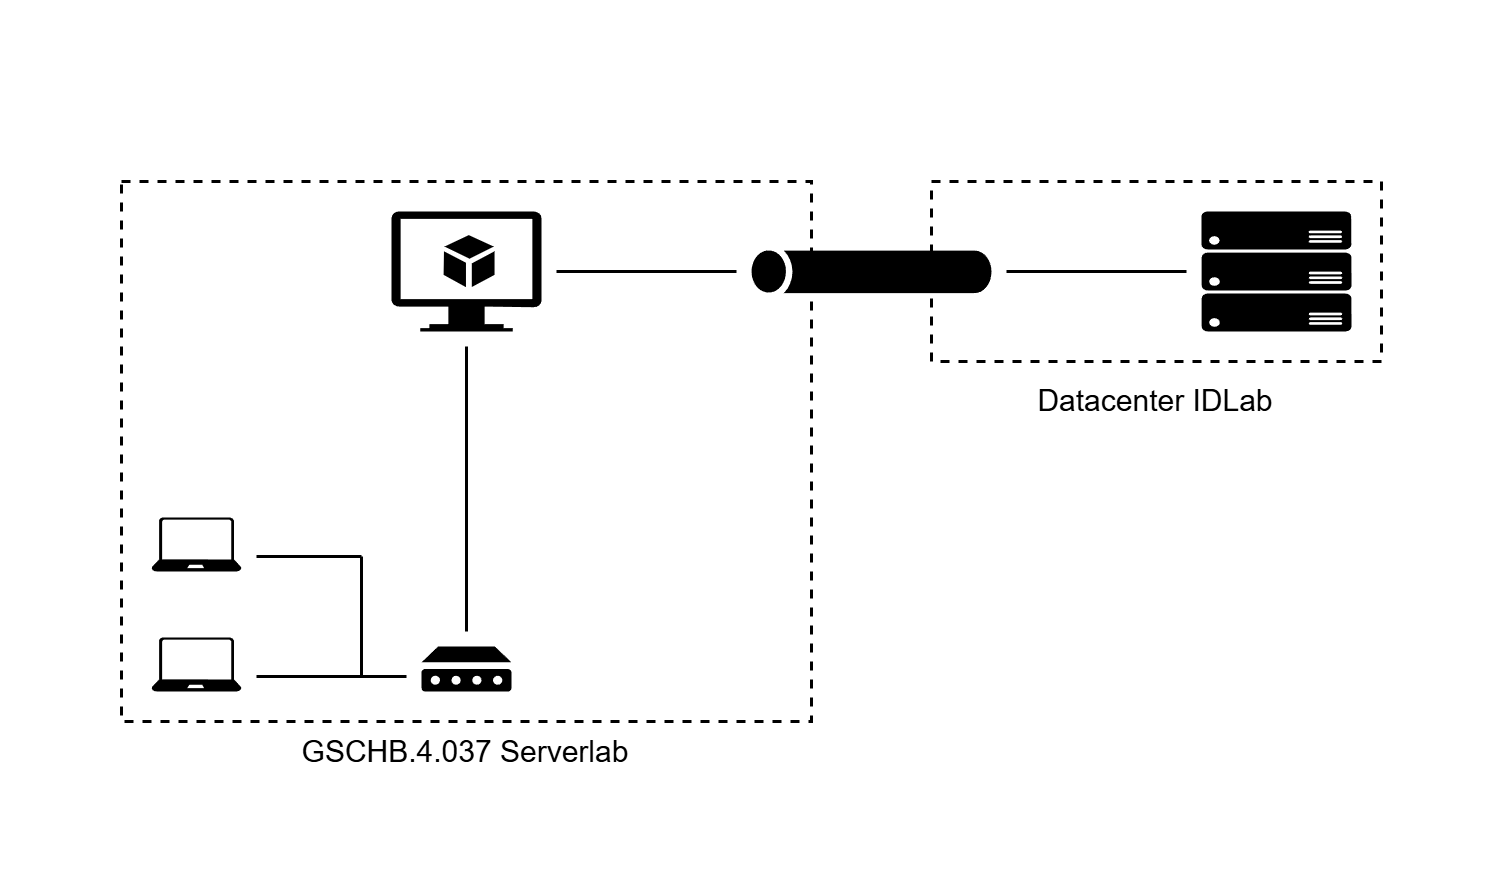
\includegraphics[width=1\textwidth]{OverzichtOpstelling.png}
    \caption[Overzicht van de opstelling.]{\label{fig:opstelling}Dit is de eerste illustratie die een beeld schetst van hoe de opstelling fundamenteel in elkaar zit.}
\end{figure}

\section{Testen van tunnels}
\label{sec:testen van tunnels}

Als tweede stap van het project wordt een vergelijkende studie uitgevoerd tussen twee tunnelingtechnologieën.  
De eenvoudigste methode is het opzetten van een Layer 2-tunnel tussen beide toestellen, waardoor ze functioneren alsof ze op hetzelfde netwerk zijn aangesloten.  
Een complexere opstelling maakt daarentegen gebruik van een combinatie van een Layer 2-verbinding en een VPN-tunnel.  

De vergelijking tussen deze twee technologieën richt zich voornamelijk op de verschillende MTU-groottes die vereist zijn voor een correcte gegevensoverdracht.  
Welke prestatieverschillen bestaan er tussen beide? Zijn ze allebei geschikt voor deze opstelling? En heeft een van de twee een duidelijke voorkeur?  

Bij deze analyse moet vooral rekening worden gehouden met de pakketgrootte om te voorkomen dat gegevensfragmentatie optreedt, aangezien beide technologieën de pakketstructuur vergroten.

\section{Automatisatie}
\label{sec:automatisatie}

Als laatste stap in het project wordt ervoor gezorgd dat de opstelling op een geautomatiseerde manier kan worden opgezet met behulp van een Ansible-playbook.  
Dit playbook is zo geschreven dat het verbinding maakt met de twee verschillende toestellen en de benodigde configuratie implementeert.  

Indien alles correct verloopt, resulteert dit in een snelle en eenvoudige oplossing om IPv6-connectiviteit te voorzien voor de labo’s die in het netwerklabo worden uitgevoerd.

% Voeg hier je eigen hoofdstukken toe die de ``corpus'' van je bachelorproef
% vormen. De structuur en titels hangen af van je eigen onderzoek. Je kan bv.
% elke fase in je onderzoek in een apart hoofdstuk bespreken.

\chapter{\IfLanguageName{dutch}{Tunnel technologieën}{Tunneling methods}}%
\label{ch:tunnel-technologieën}

\section{deel 1}
\label{sec:deel1}
\chapter{\IfLanguageName{dutch}{Automatisatie}{Automatisation}}%
\label{ch:automatisatie}

\section{deel 1}
\label{sec:deel1}
%...

%%=============================================================================
%% Conclusie
%%=============================================================================

\chapter{Conclusie}%
\label{ch:conclusie}

% TODO: Trek een duidelijke conclusie, in de vorm van een antwoord op de
% onderzoeksvra(a)g(en). Wat was jouw bijdrage aan het onderzoeksdomein en
% hoe biedt dit meerwaarde aan het vakgebied/doelgroep? 
% Reflecteer kritisch over het resultaat. In Engelse teksten wordt deze sectie
% ``Discussion'' genoemd. Had je deze uitkomst verwacht? Zijn er zaken die nog
% niet duidelijk zijn?
% Heeft het onderzoek geleid tot nieuwe vragen die uitnodigen tot verder 
%onderzoek?

Nog niet van toepassing. (Work in progress)



%---------- Bijlagen -----------------------------------------------------------

\appendix

\chapter{Onderzoeksvoorstel}

Het onderwerp van deze bachelorproef is gebaseerd op een onderzoeksvoorstel dat vooraf werd beoordeeld door de promotor. Dat voorstel is opgenomen in deze bijlage.

%% TODO: 
%\section*{Samenvatting}

% Kopieer en plak hier de samenvatting (abstract) van je onderzoeksvoorstel.

% Verwijzing naar het bestand met de inhoud van het onderzoeksvoorstel
%---------- Inleiding ---------------------------------------------------------

% TODO: Is dit voorstel gebaseerd op een paper van Research Methods die je
% vorig jaar hebt ingediend? Heb je daarbij eventueel samengewerkt met een
% andere student?
% Zo ja, haal dan de tekst hieronder uit commentaar en pas aan.

\paragraph{Opmerking}

Dit voorstel is gebaseerd op het onderzoeksvoorstel dat werd geschreven in het
kader van het vak Research Methods dat ik vorig academiejaar heb
uitgewerkt met \\ Maarten Adriaenssens als mede-auteur.


\section{Inleiding}%
\label{sec:inleiding}

Door de implementatie van IPv6 kan een netwerk snel futureproof gemaakt worden, het is een relatief nieuwe technologie die het probleem van de gelimiteerde 32-bit adressen in IPv4 oplost
door gebruik te maken van 128-bit adressen. Hoewel deze technologie al sinds 1998 bestaat, blijft de toepassing ervan beperkt. 
Dit blijkt duidelijk uit de IPv6 Support Rate-grafiek zoals gezien op de website van \textcite{EuropeanCommission}, 
waaruit blijkt dat in België aan het begin van 2024 59\% van de eindgebruikers toegang heeft tot de technologie, 
terwijl slechts 29\% van de services compatibel zijn met IPv6.\\

SmartEye wil ervoor zorgen dat het Eduroam-netwerk, dat ze hebben opgezet en onderhouden, de nodige upgrade krijgt en zoekt daarvoor een geautomatiseerde oplossing. 
Een eerste probleem hierbij is dat de netwerken die zijn uitgebouwd, 
niet allemaal op dezelfde manier functioneren. De netwerkapparatuur die is geïnstalleerd bestaat uit onder andere Cisco- en MikroTik-apparatuur, 
waarbij elk toestel op een andere manier moet worden geconfigureerd.  
De configuratie van een MikroTik-toestel vereist eerst een certificaat, dat door SmartEye zelf wordt voorzien voor de uitwerking van deze proef. 
Een dual-stack netwerk heeft de voorkeur, omdat dit geïmplementeerd kan worden zonder het risico dat bestaande opstellingen niet werken. 
Daarnaast zal NAT64 aan bod komen om toestellen die IPv6 niet ondersteunen toch te laten communiceren met het netwerk. Dit alles draagt bij aan de robuustheid ervan, 
aangezien beide technologieën dan op alle plaatsen gebruikt kunnen worden. \\

Het doel van de proef is om een algemeen script te ontwikkelen dat gebruikt kan worden om alle netwerktoestellen binnen het Eduroam-netwerk voor te bereiden op het gebruik van het nieuw verkregen IPv6-adres. 
Dit script zal niet alleen op de externe toestellen worden toegepast, maar ook op de backbone van SmartEye zelf. 
De ontwikkeling van het script zal plaatsvinden in een labo-omgeving die door SmartEye is voorzien.

%---------- Stand van zaken ---------------------------------------------------

\section{Literatuurstudie}%
\label{sec:literatuurstudie}

\subsection{Implementatie}
\label{sec:implementatie}

Zoals eerder vermeld is de implementatie van IPv6 beperkt. 
Dit terwijl marktleiders van internet service providers zoals Cloudflare, Proximus en Telenet dicht tegen de 100\% zitten op het vlak van aangeboden IPv6 percentage \autocite{Test2024}. 
Ook op de website van \textcite{EuropeanCommission} is zichtbaar dat op vlak van end-user implementatie België deel van de marktleiders is, terwijl de services nog geen 30\% haalt.

\subsection{Netwerk-configuratie via Ansible}
\label{sec:netconfigAnsible}

Een geautomatiseerde uitrol van netwerkconfiguraties kan worden uitgevoerd met Ansible, waarbij onderscheid moet worden gemaakt tussen de merken netwerkapparatuur. 
Hiervoor zal de configuratie worden opgesplitst in apparte YAML-bestanden, die in het Ansible-playbook worden aangeroepen.\\
Deze YAML-bestanden bevatten minstens de volgende componenten: functies voor het instellen van IPv6-adressen op de interfaces, 
de juiste configuratie van de loopback-interface, en de minimale configuratie voor EIGRP of OSPF \autocite{MohdFuziMohdFaris2021}.

\subsection{IPv4 vs IPv6}
\label{sec:IPv4vsIPv6}

Met de huidige snelheid waarmee het internet groeit en evolueert, wordt het duidelijker dat de huidige toewijzing van IP-adressen het tempo niet zal kunnen bijhouden. 
Zelfs met technologieën zoals CIDR1 en NAT2 zal dit probleem niet worden opgelost, alleen uitgesteld \autocite{Gu2005}.
Gelukkig bestaat er al een andere oplossing: het gebruik van IPv6, aangezien dit 128 bits gebruikt voor zijn adresseringsformaat in plaats van de 32 bits van IPv4. 
De huidige netwerkinfrastructuren bieden verschillende manieren om IPv6 te implementeren: dual-stack, tunneling of vertaling \autocite{Zunainah2021}. 
Deze implementatiemethoden hebben elk hun eigen voordelen en nadelen. De keuze is sterk afhankelijk van de huidige netwerktopologie en -infrastructuur. 
Hoewel op het eerste gezicht een dual-stack de oplossing lijkt, moet er verder onderzoek worden gedaan om de optimale keuze te bepalen \autocite{Zehl2001}.

% Voor literatuurverwijzingen zijn er twee belangrijke commando's:
% \autocite{KEY} => (Auteur, jaartal) Gebruik dit als de naam van de auteur
%   geen onderdeel is van de zin.
% \textcite{KEY} => Auteur (jaartal)  Gebruik dit als de auteursnaam wel een
%   functie heeft in de zin (bv. ``Uit onderzoek door Doll & Hill (1954) bleek
%   ...'')

%---------- Methodologie ------------------------------------------------------
\section{Methodologie}%
\label{sec:methodologie}

\subsection{Voorbereiding}
\label{sec:voorbereiding}
{\small Duurtijd : 2 - 3 Weken}\\

Aangezien een groot deel van de toestellen afkomstig is van MikroTik, zal er eerst een bijscholing plaatsvinden waarin een certificaat wordt behaald. 
Na het behalen van dit certificaat zal er een overleg plaatsvinden met de co-promotor om de opdracht verder toe te lichten. 
Hierbij wordt bepaald welke toestellen geconfigureerd moeten worden en op welke manier dit moet gebeuren.\\

Om de scripts te kunnen schrijven voor de verschillende toestellen, zal uitgebreide documentatie verzameld worden. 
Daarnaast worden de benodigde beveiligingsmaatregelen besproken en indien mogelijk in de configuratie verwerkt.\\

Tot slot wordt vastgesteld welke IPv6-adressen aan welke gebruikers worden toegewezen en welke adressen of reeksen gereserveerd blijven voor specifieke doeleinden.

\subsection{Ontwerp}
\label{sec:ontwerp}
{\small Duurtijd : 3 - 4 Weken}\\

De uitwerking van het script gebeurt via een Ansible Playbook, dat gebruikmaakt van verschillende YAML-bestanden om een opsplitsing te maken tussen de verschillende types toestellen.
Het playbook is een zelfgeschreven verzameling van bestanden die alle nodige voorzieningen bevat en de benodigde toestellen configureert. De configuraties zijn daarbij opgesplitst in afzonderlijke taken.

\subsection{Testing}
\label{sec:testing}
{\small Duurtijd : 3 - 4 Weken}\\

Het testen van dit script zal plaatsvinden in een labo-omgeving. In het eerste stadium worden virtuele machines op de testservers gebruikt als een soort 'sandbox'.
Deze omgeving zal dan ook gebruikt worden als een proof of concept.
Indien alles daar goed verloopt, kan er worden overgegaan naar de volgende stap.
Bij foutmeldingen of problemen zal contact worden opgenomen met de co-promotor. Voor eenvoudige fouten kan ook gebruik worden gemaakt van online bronnen om een oplossing te vinden.

\subsection{Deployment}
\label{sec:deployment}
{\small Duurtijd : 2 - 4 Weken}\\

De uitrol van het script verloopt in verschillende stadia. 
Zodra alles is goedgekeurd in de testomgeving, wordt als eerste gekeken naar de overgang van de backbone van het bedrijf naar IPv6.
Dit is de eerste stap omdat de backbone uit een groot aantal merken netwerkapparatuur bestaat, wat een bredere testbasis biedt.\\

Na de implementatie op de backbone wordt de focus verlegd naar kleine particuliere netwerken. 
Dit stadium heeft een lager risico, waardoor eventuele problemen makkelijker op te lossen zijn voordat grotere implementaties plaatsvinden.\\

In het laatste stadium worden de grote locaties aangepakt, zoals onderwijsinstellingen en grote studentenkoten. 
Voor deze implementatie is eerst overleg nodig met de netwerkverantwoordelijken van de locaties om een probleemloze overgang te garanderen.

%---------- Verwachte resultaten ----------------------------------------------
\section{Verwacht resultaat, conclusie}%
\label{sec:verwachte_resultaten}

De implementatie van een geautomatiseerde methode voor de overgang naar IPv6 op het Eduroam-netwerk heeft aangetoond 
dat een netwerk met verschillende netwerkapparatuur een uitgebreid stappenplan vereist. 
Het is daarbij essentieel om een duidelijk onderscheid te maken tussen de verschillende vereisten van de gebruikte apparatuur.

De belangrijkste resultaten zijn:
\begin{itemize}
    \item Een robuust script dat kan gebruikt worden voor de verschillende merken van netwerkapparatuur.
    \item Een overgang voor alle klanten van SmartEye naar IPv6 waarbij hoofdzakelijk op een dualstack wijze gewerkt is.
    \item Een script dat foutbestendig is en dat een bestaand netwerk niet uitschakelt.
\end{itemize}

De testfase in de labo-omgeving heeft de efficiëntie van de scripts getoond en de uitrol op de backbone van SmartEye heeft de betrouwbaarheid van het netwerk bevestigd. 
Dit biedt een basis voor de verdere implementatie op externe locaties van nieuwe klanten/gebruikers van het Eduroam netwerk.


%%---------- Andere bijlagen --------------------------------------------------
% TODO: Voeg hier eventuele andere bijlagen toe. Bv. als je deze BP voor de
% tweede keer indient, een overzicht van de verbeteringen t.o.v. het origineel.
%\input{...}

%%---------- Backmatter, referentielijst ---------------------------------------

\backmatter{}

\setlength\bibitemsep{2pt} %% Add Some space between the bibliograpy entries
\nocite{*}
\printbibliography[heading=bibintoc]

\end{document}
